\documentclass[11pt]{article}



\usepackage[a4paper,margin=2.5cm]{geometry}

\usepackage[utf8]{inputenc}
\usepackage[T1]{fontenc}
\usepackage[brazil]{babel}

\usepackage{setspace}
\doublespacing



\usepackage{amsmath}
\usepackage{amssymb}
\usepackage{mathtools}
\usepackage{IEEEtrantools}



\usepackage{graphicx}
\graphicspath{{./Secoes/Figuras/Photos/}}

\usepackage{float}
\usepackage{booktabs}
\usepackage{multirow}
\usepackage[table]{xcolor}
\usepackage{adjustbox}



\usepackage[ruled,vlined,linesnumbered]{algorithm2e}



\usepackage{caption}
\captionsetup{
    justification=raggedright,
    singlelinecheck=false
}

\usepackage{subcaption}



\usepackage{tikz}
\usetikzlibrary{positioning, arrows.meta}

\usepackage{pgfgantt}



\usepackage{xcolor}

\newcommand{\blue}[1]{\textcolor{blue}{#1}}
\newcommand{\red}[1]{\textcolor{red}{#1}}

\usepackage[hidelinks]{hyperref}



\setlength{\parindent}{1.25cm}
\setlength{\parskip}{4pt}



\usepackage{csquotes}
\usepackage{multicol}
\usepackage[backend=biber,bibstyle=ieee,citestyle=numeric,sorting=none,sortcites=true,doi=true,isbn=true,url=true,natbib=true]{biblatex}
\addbibresource{Secoes/Referencias/referencias.bib}

\setlength{\bibitemsep}{0.25\baselineskip}
\setlength{\bibhang}{1em}
\setlength{\biblabelsep}{0.5em}



\begin{document}

\newcommand{\conjuntoItens}{

\begin{tikzpicture}[
    thick,
    item/.style={circle, draw, minimum size=9mm},
    buyer/.style={circle, draw,  minimum size=9mm}
]
\node[item] (i1) at (0,2) {$i_1$};
    \node[item] (i2) at (0,0) {$i_2$};
    \node[item] (i3) at (0,-2) {$i_3$};
    \node[item] (i3) at (0,-4) {$i_4$};

\end{tikzpicture}
}


\newcommand{\conjuntoCompradores}{

\begin{tikzpicture}[
    thick,
    item/.style={circle, draw, minimum size=9mm},
    buyer/.style={circle, draw,  minimum size=9mm}
]

\node[buyer] (b1) at (5,2) {$b_1$};
    \node[buyer] (b2) at (5,0) {$b_2$};
    \node[buyer] (b2) at (5,-2) {$b_3$};
    \node[buyer] (b2) at (5,-4) {$b_4$};

\end{tikzpicture}
}


\newcommand{\conjuntoItensValorados}{

\begin{tikzpicture}[
    thick,
    item/.style={circle, draw, minimum size=9mm},
    buyer/.style={circle, draw,  minimum size=9mm},
    scale=0.8
]
\node[item] (i1) at (0,2) {$i_1$};
    \node[item] (i2) at (0,0) {$i_2$};
    \node[item] (i3) at (0,-2) {$i_3$};
    \node[item] (i4) at (0,-4) {$i_4$};

\node[buyer] (b1) at (5,2) {$b_1$};
    \node[buyer] (b2) at (5,0) {$b_2$};
    \node[buyer] (b3) at (5,-2) {$b_3$};
    \node[buyer] (b4) at (5,-4) {$b_4$};

\draw (b1) --node[pos=0.2, fill=white]{3} (i1);
    \draw (b1) --node[pos=0.2, fill=white]{4} (i2);
    \draw (b1) --node[pos=0.2, fill=white]{2} (i3);

    \draw (b2) --node[pos=0.2, fill=white]{5} (i2);
    \draw (b2) --node[pos=0.2, fill=white]{6} (i3);
    \draw (b2) --node[pos=0.2, fill=white]{3} (i4);

    \draw (b3) --node[pos=0.2, fill=white]{5} (i3);
    \draw (b3) --node[pos=0.2, fill=white]{2} (i4);

    \draw (b4) --node[pos=0.2, fill=white]{2} (i4);
\end{tikzpicture}
}

\newcommand{\conjuntoItensPrecificados}{

\begin{tikzpicture}[
    thick,
    item/.style={circle, draw, minimum size=9mm},
    buyer/.style={circle, draw,  minimum size=9mm},
    scale=0.8
]
\node[item, label=below:{$p_1 = 3$}] (i1) at (0,2) {$i_1$};
    \node[item, label=below:{$p_2 = 5$}] (i2) at (0,0) {$i_2$};
    \node[item, label=below:{$p_3 = 5$}] (i3) at (0,-2) {$i_3$};
    \node[item, label=below:{$p_4 = 3$}] (i4) at (0,-4) {$i_4$};

\node[buyer] (b1) at (5,2) {$b_1$};
    \node[buyer] (b2) at (5,0) {$b_2$};
    \node[buyer] (b3) at (5,-2) {$b_3$};
    \node[buyer] (b4) at (5,-4) {$b_4$};

\draw (i1) -- (b1);
    \draw (i4) -- (b2);
    \draw (i3) -- (b3);
    
\end{tikzpicture}
}


\newcommand{\fluxograma}{
    \begin{tikzpicture}[
        every node/.style={draw, minimum height=1.2cm, minimum width=3.8cm, font=\ttfamily, align=center},
        decision/.style={aspect=2, draw, minimum height=1.5cm, inner sep=0pt},
        arrow/.style={->, thick},
        node distance=1.2cm and 2cm
    ]
\node (begin) at (-10,-1.5) [circle, draw, minimum size=1.2cm] {Início};
        \node (genKeys) at (-5,-1.5) {Gerar a população\\ inicial};
        \node (fitness) at (-5, -4) {Avaliação de \\ fitness};
        \node (checkStop) at (4, -4) [diamond, decision, fill=gray!20] {Critério de parada\\ satisfeito?};
        \node (selection) at (4, -8) {Seleção};
        \node (crossover) at (-1.5, -8) {Cruzamento};
        \node (mutation) at (-7.5, -8) {Mutação};
        \node (elitism) at (-13.5, -8) {Elitismo};
        \node (newPop) at (-13.5, -4) {Nova população};
        \node (final) at (4, -1) [circle, draw, minimum size=1.2cm] {Fim};
        
    \begin{scope}[
              every node/.style={fill=white,circle}, arrow/.style={->,ultra thick}]
\draw[arrow] (begin) -- (genKeys);
        \draw[arrow] (genKeys) -- (fitness);
        \draw[arrow] (fitness) -- (checkStop);
        \draw[arrow] (checkStop) --node[right]{Não} (selection);
        \draw[arrow] (selection) -- (crossover);
        \draw[arrow] (crossover) -- (mutation);
        \draw[arrow] (mutation) -- (elitism);
        \draw[arrow] (elitism) -- (newPop);
        \draw[arrow] (newPop) -- (fitness);
        \draw[arrow] (checkStop) -- node[right]{Sim} (final);
        
    \end{scope}
    \end{tikzpicture}
}

\newcommand{\fluxogramaBRKGA}{
    \begin{tikzpicture}[
        every node/.style={draw, minimum height=1.2cm, minimum width=3.8cm, font=\ttfamily, align=center},
        decision/.style={aspect=2, draw, minimum height=1.5cm, inner sep=0pt},
        arrow/.style={->, thick},
        node distance=1.2cm and 2cm
    ]
\node (begin) at (-10,-1.5) [circle, draw, minimum size=1.2cm] {Início};
        \node (genKeys) at (-5,-1.5) {Gerar os vetores\\ de chaves aleatórias};
        \node (fitness) at (-5, -4) {Decodificar cada vetor \\ de chave aleatória};
        \node (checkStop) at (4, -4) [diamond, decision, fill=gray!20] {Regra de parada\\ satisfeito?};
        \node (selection) at (4, -8) {Classificar indivíduos\\como elite ou não-elite};
        \node (crossover) at (-2, -8) {Copiar os elite para\\a próxima geração};
        \node (mutation) at (-7.5, -8) {Criar mutantes para\\próxima geração};
        \node (elitism) at (-13.5, -8) {Gerar descendentes para\\a próxima geração};
        \node (newPop) at (-13.5, -4) {Nova população};
        \node (final) at (4, -1) [circle, draw, minimum size=1.2cm] {Fim};
        
    \begin{scope}[
              every node/.style={fill=white,circle}, arrow/.style={->,ultra thick}]
\draw[arrow] (begin) -- (genKeys);
        \draw[arrow] (genKeys) -- (fitness);
        \draw[arrow] (fitness) -- (checkStop);
        \draw[arrow] (checkStop) --node[right]{Não} (selection);
        \draw[arrow] (selection) -- (crossover);
        \draw[arrow] (crossover) -- (mutation);
        \draw[arrow] (mutation) -- (elitism);
        \draw[arrow] (elitism) -- (newPop);
        \draw[arrow] (newPop) -- (fitness);
        \draw[arrow] (checkStop) -- node[right]{Sim} (final);
        
    \end{scope}
    \end{tikzpicture}
}
 
{
        \centering
    
        {\large Universidade Estadual de Campinas \\}
        {\large Instituto de Computação \\[2cm]}
        
        {\LARGE \textbf{O Problema da Compra Mínima: Formulações e Heurísticas} \\[2cm]}
        
        {\large Candidato: Antônio Erick Freitas Ferreira \\}

        {\large Orientador: Rafael Crivellari Saliba Schouery}
        
    }

    \begin{abstract}

O problema de determinar preços estratégicos para um conjunto de produtos constitui um desafio central em cenários de mercados competitivos, gerando um dilema econômico difícil: preços elevados maximizam a receita unitária, mas restringem o mercado consumidor, enquanto preços baixos expandem o volume de vendas em detrimento da margem de lucro por transação. Diante disso, este trabalho aborda o Problema da Compra Mínima (PCmin), no qual um vendedor busca maximizar sua receita total ao estipular preços para um conjunto de itens ofertados a um conjunto de compradores, cujas valorações e disposições máximas a pagar são conhecidas. Além disso, o comportamento dos consumidores é assumido sob a hipótese de demanda unitária, de modo que cada comprador adquire estritamente o item viável de menor preço disponível ou opta por não comprar nenhum produto caso todos excedam sua valoração. Na literatura, o PCmin tem sido pouco explorado sob a perspectiva de algoritmos exatos, e tais resultados computacionais possibilitam oportunidades substanciais de aprimoramento, em particular no desenvolvimento de métodos capazes de tratar instâncias de grande porte em tempos computacionais viáveis. Portanto, este projeto tem como objetivo propor formulações matemáticas fortalecidas de Programação Linear Inteira e desenvolver abordagens heurísticas baseadas nos \emph{frameworks} BRKGA e RKO, visando obter soluções eficientes e escaláveis para o problema.

\end{abstract}

 
    {\textbf{Palavras-chave:} Otimização combinatória, precificação, programação linear inteira, heurística.}
%
 
\newpage



\section{Introdução}

No comércio, decidir o preço de um produto deixou de ser uma tarefa simples para se tornar uma estratégia essencial para aumentar o faturamento. Esse desafio define os \emph{Problemas de Precificação} (PP), onde o vendedor precisa encontrar valores que maximizem sua receita total, equilibrando o preço de cada item com o interesse dos clientes em comprá-lo~\cite{smith1986}. Dado importância prática, esse tema é muito estudado e aparece em diversos setores da economia~\cite{aggarwal2004,venkatesan2005,shmuel1984,shmuel1987,smith1986}.

Rusmevichientong et al.~\cite{rusmevichientong2006} estabeleceram um modelo geral para a precificação de múltiplos itens, onde o vendedor conhece quanto cada cliente está disposto a pagar e busca a maior receita possível. A partir dessa base, surgem diferentes modelos de comportamento. No \textit{Problema da Compra Máxima} (PCmax), o cliente escolhe o item mais caro que pode pagar, enquanto no \textit{Problema da Compra por Preferência} (PCrank), a escolha segue uma ordem de prioridade pessoal.

Já no Problema da Compra Mínima (PCmin), o foco deste projeto, assume-se que o comprador levará o item mais barato entre aqueles que ele considera viáveis. Essa última premissa reflete situações reais onde o consumidor busca a opção mais econômica entre substitutos aceitáveis, tornando o PCmin um cenário de grande relevância prática.

De maneira formal, o PCmin foi definido por Rusmevichientong et al.~\cite{rusmevichientong2006} da seguinte forma. Seja $I$ um conjunto de itens com estoque ilimitado e $B$ um conjunto de compradores. As preferências dos consumidores são representadas por uma matriz de valorações~$V = \{v_{ib} \mid v_{ib} \in \mathbb{R}_+\}$, em que cada elemento $v_{ib}$ corresponde ao valor máximo que o comprador $b \in B$ está disposto a pagar pelo item $i \in I$. Caso um comprador não tenha interesse em determinado item, sua valoração correspondente é definida como zero.

O objetivo do problema consiste em determinar um vetor de preços não negativos~$P = \{p_i \mid p_i \in \mathbb{R}_+\}$, atribuindo a cada item $i \in I$ um preço $p_i$, de modo a maximizar a receita total do vendedor. Além disso, assume-se que o comportamento dos compradores é determinístico e orientado exclusivamente pelos preços praticados. Assim, cada comprador $b \in B$ considera apenas os itens viáveis para seu orçamento, isto é, aqueles cujo preço satisfaz $p_i \leq v_{ib}$, e adquire o item de menor preço entre eles. Formalmente, o comprador $b$ escolhe um item $i \in I$ tal que~$p_i \leq v_{ib}$ e, para qualquer outro item $j \in I$ que satisfaça $p_j \leq v_{jb}$, tem-se $p_i \leq p_j$. Caso não exista nenhum item viável para o comprador, nenhuma compra é realizada.


A Figura~\ref{fig:exemploPCmin} apresenta um exemplo ilustrativo de uma instância do PCmin. Na subfigura~(a), são representadas as relações de valoração entre os itens e os compradores por meio de um grafo bipartido, no qual cada aresta ponderada indica a valoração atribuída por um comprador a um determinado item. Na subfigura~(b), são mostrados os preços atribuídos aos itens e as escolhas induzidas pela suposição do comportamento. Nesse caso, o comprador adquire a opção mais barata de seu interesse, desde que o valor não exceda sua valoração. Assim, observa-se que o comprador $b_1$ seleciona o item $i_1$, o comprador $b_2$ seleciona o item $i_4$, o comprador $b_3$ seleciona o item $i_3$, enquanto o comprador $b_4$ não realiza compra, uma vez que não há item viável disponível para ele.

\begin{figure}[H]
\centering

\begin{subfigure}[t]{0.45\textwidth}
    \centering
    \conjuntoItensValorados
    \caption{Relações de valoração entre itens e compradores, representadas pelas arestas ponderadas da matriz $V$.}
\end{subfigure}
\hfill
\begin{subfigure}[t]{0.45\textwidth}
    \centering
    \conjuntoItensPrecificados
    \caption{Preços atribuídos aos itens e seleção induzida dos compradores segundo a regra do PCmin.}
\end{subfigure}

\caption{Exemplo ilustrativo de uma instância do PCmin, com as valorações entre itens e compradores e a seleção induzida pelos preços atribuídos.}
\label{fig:exemploPCmin}
\end{figure}

No exemplo ilustrado na Figura~\ref{fig:exemploPCmin}, a solução apresentada gera uma receita total de 11 unidades monetárias, correspondente às compras realizadas por $b_1$, $b_2$ e $b_3$. Entretanto, esse conjunto de preços não é necessariamente ótimo. Alterações nos preços podem modificar o conjunto de itens viáveis para cada comprador e, consequentemente, alterar tanto a quantidade de vendas quanto a receita obtida por item. Assim, a definição dos preços envolve uma interação não trivial entre viabilidade de compra e retorno financeiro, o que justifica o uso de métodos de otimização para a resolução do PCmin.

No que se refere ao desenvolvimento teórico do PCmin, Rusmevichientong et al.~\cite{rusmevichientong2006} foram os primeiros a formalizar o Pcmin e outras variantes, como o PCmax e o PCrank, no contexto de problemas de precificação com múltiplos itens e compradores. Esse estudo possui caráter predominantemente conceitual, concentrando-se na definição do problema e em suas propriedades estruturais. Posteriormente, Briest e Krysta~\cite{briest2007} e Chalermsook et al.~\cite{chalermsook2012} aprofundaram a investigação teórica do PCmin ao estabelecer resultados de complexidade e aproximabilidade, evidenciando sua elevada dificuldade computacional. Esses trabalhos são fundamentais por consolidarem o entendimento de que o problema é NP-difícil e, portanto, desafiador sob a perspectiva algorítmica. 

Mais recentemente, Catabriga~\cite{catabriga2025} estudou o PCmin sob a ótica da otimização exata, propondo diferentes formulações de Programação Linear Inteira (PLI) e Programação Linear Inteira Mista (PLIM), como também de técnicas de fortalecimento para tais formulações. Embora os resultados mostrem o potencial dessas abordagens, também revelam limitações de escalabilidade para instâncias maiores. Além disso, até o momento, não foram identificadas na literatura heurísticas focadas em cenários de grande porte (em especial com mais de 1000 itens ou compradores), o que aponta uma lacuna importante no tratamento do problema.

Este trabalho posiciona-se como uma continuidade dessa linha de pesquisa. O primeiro objetivo é aperfeiçoar os modelos PLIM existentes para o PCmin por meio do fortalecimento da relaxação linear, eliminação de simetrias, redução de variáveis e restrições, além de reformulações que favoreçam o desempenho de solucionadores como o Gurobi~\cite{gurobi}. Já no segundo objetivo, busca-se desenvolver heurísticas eficientes para obter soluções de alta qualidade para instâncias grandes em tempo reduzido. Espera-se, assim, ampliar as ferramentas disponíveis para resolver o PCmin, tanto no âmbito de métodos exatos quanto no de abordagens heurísticas. 
\section{Trabalhos Relacionados}

O PCmin integra uma classe fundamental de problemas de precificação de múltiplos itens com restrições de demanda, cujas fundações teóricas e matemáticas apoiam-se em modelos de comportamento do consumidor amplamente consolidados na literatura de otimização combinatória. A formalização geral desse ecossistema de precificação foi estabelecida por Rusmevichientong et al.~\cite{rusmevichientong2006}, que estruturaram o cenário onde um vendedor busca maximizar sua receita conhecendo a disposição máxima a pagar de cada cliente. Dentro dessa mesma árvore conceitual, o \emph{Problema da Compra Máxima} (PCmax), proposto originalmente por Aggarwal et al.~\cite{aggarwal2004}, adota uma premissa de comportamento inversa ao do PCmin: assume-se que o comprador, diante das opções viáveis, seleciona sempre o item de maior valor absoluto. Variando essa dinâmica de escolha, o \emph{Problema da Compra por Preferência} (PCrank) modela cenários onde o consumidor segue uma lista estrita de prioridades pessoais. Embora os critérios de seleção variem entre essas vertentes, as estruturas algorítmicas desenvolvidas para eles apoiam indiretamente o avanço do PCmin; a formulação de decisão indireta (DIB), por exemplo, foi originalmente concebida e validada no contexto do PCmax por Aggarwal et al.~\cite{aggarwal2004} antes de ser adaptada para a regra de escolha pelo menor preço.

Outro pilar teórico para a modelagem matemática do PCmin é o conceito de \emph{Precificação Livre de Inveja} (do inglês, \emph{Envy-Free Pricing}), introduzido no campo da otimização algorítmica por Guruswami et al.~\cite{venkatesan2005}. Nessa variante, os preços determinados para os produtos devem garantir um equilíbrio de mercado onde nenhum comprador prefira o feixe de itens alocado a outro indivíduo em detrimento do seu próprio. O modelo linear inteiro misto clássico para o cenário livre de inveja, inicialmente formalizado por Heilporn et al.~\cite{heilporn2010} e expandido por Fernandes et al.~\cite{fernandes2016}, serve como base direta para a criação da formulação de Decisão Direta (DD) utilizada no PCmin.

Especificamente sobre o avanço do PCmin, Briest e Krysta~\cite{briest2007} e Chalermsook et al.~\cite{chalermsook2012} solidificaram a investigação teórica ao mapear os limites de complexidade e aproximabilidade do problema, demonstrando que ele é NP-difícil e altamente desafiador sob a perspectiva algorítmica. Além disso, recentemente Catabriga~\cite{catabriga2025} realizou o primeiro estudo focado na otimização exata do PCmin, propondo formulações matemáticas inteiras e mistas e investigando técnicas para o fortalecimento de seus limites lineares. Todavia, os experimentos dessa pesquisa pioneira evidenciaram barreiras de escalabilidade para instâncias de grandes dimensões e apontaram uma lacuna completa na literatura no que tange ao desenvolvimento de abordagens heurísticas focadas em cenários de grande porte. Dessa forma, as investigações e desenvolvimentos prévios sobre o PCmax, o PCrank e a precificação livre de inveja fornecem um arsenal metodológico que fundamenta o fortalecimento de modelos e a criação de heurísticas escaláveis propostos neste projeto. 
\section{Metodologia}

A presente seção descreve a metodologia adotada para o desenvolvimento deste trabalho. Inicialmente, são apresentados os conceitos de Programação Linear e Programação Linear Inteira. Em seguida, são discutidas metaheurísticas inspiradas em processos evolutivos, com ênfase nos Algoritmos Genéticos e em suas variações baseadas em chaves aleatórias. Depois, é introduzido o \emph{framework} Random-Key Optimizer (RKO)~\cite{Chaves2023}. Por fim, são discutidas as formulações matemáticas existentes para o PCmin.

\subsection{Programação Linear}

A \textit{Programação Linear} (PL) é uma das técnicas centrais da Otimização Combinatória, aplicada na modelagem e resolução de problemas de otimização onde funções lineares representam tanto o objetivo quanto as restrições do sistema~\cite{Goldbarg2005}.

Em um modelo de PL, assume-se que as variáveis de decisão pertencem ao conjunto dos números reais $\mathbb{R}$, isto é, são contínuas. As restrições do modelo delimitam a região viável, e uma solução é considerada viável se satisfaz todas essas restrições. Uma solução ótima corresponde a uma solução viável que maximiza (ou minimiza) a função objetivo. Quando expresso em sua forma canônica, o modelo de programação linear pode ser descrito como:

\[
    \begin{aligned}
    &\text{maximize} \quad  z  = &c^T x \\
    &\text{sujeito a} \quad & Ax & \leq & b \\
    & & x & \geq & 0
    \end{aligned}
\]

em que:
\begin{itemize}
    \item $x \in \mathbb{R}^n$ representa o vetor de variáveis de decisão;
    \item $c \in \mathbb{R}^n$ contém os coeficientes da função objetivo;
    \item $A \in \mathbb{R}^{m \times n}$ é a matriz de coeficientes das restrições;
    \item $b \in \mathbb{R}^m$ representa os termos independentes das restrições;
    \item $z \in \mathbb{R}$ é o valor da função objetivo.
\end{itemize}

Um dos principais avanços na resolução de problemas de PL ocorreu em 1947, quando George Dantzig propôs o algoritmo \emph{simplex}~\cite{Nash2000}. Trata-se de um método exato e iterativo que explora a estrutura geométrica do problema, percorrendo os vértices do politopo definido pelas restrições. A cada iteração, o método busca um vértice adjacente que melhore o valor da função objetivo, até que não seja mais possível obter ganhos adicionais, caracterizando assim a otimalidade da solução correspondente ao vértice atual~\cite{Goldbarg2005}.

Embora o método simplex apresente uma eficiência prática notável, resolvendo a maioria dos problemas reais em um número de iterações linear em relação ao número de restrições, sua complexidade teórica no pior caso é exponencial~\cite{klee1972}. Esse comportamento ocorre porque, em instâncias específicas, o algoritmo pode ser forçado a percorrer todos os vértices do politopo antes de alcançar a solução ótima.

Essa limitação teórica motivou a busca por algoritmos de tempo polinomial. O primeiro marco nessa direção foi o método dos elipsoides, proposto por Leonid Khachiyan~\cite{khachiyan1979}, que provou matematicamente que a programação linear pertence à classe de complexidade polinomial. Contudo, apesar de seu valor teórico histórico, o método dos elipsoides mostrou-se computacionalmente ineficiente e lento para resolver instâncias práticas.

O cenário mudou significativamente em 1984, quando Narendra Karmarkar~\cite{karmarkar1984} introduziu o método de pontos interiores, um algoritmo que combina complexidade teórica polinomial com um desempenho prático altamente competitivo. Diferentemente do simplex, que caminha pela fronteira do politopo através de seus vértices, os métodos de pontos interiores (e suas variações modernas, como os algoritmos de barreira primal-dual) cruzam o interior da região viável em direção a uma solução ótima. Atualmente, os principais \emph{solvers} comerciais utilizam tanto o algoritmo simplex quanto os métodos de barreira e pontos interiores, escolhendo a abordagem mais adequada a depender da estrutura e da escala do problema linear a ser resolvido.

\subsubsection{Programação Linear Inteira}

A \textit{Programação Linear Inteira} (PLI) e a sua variante Mista (PLIM) estendem a PL ao impor que a totalidade ou parte das variáveis de decisão assumam valores discretos~\cite{Nemhauser1988}. Embora matematicamente simples, alterar o espaço de soluções de contínuo para discreto torna a resolução de tais modelos um problema NP-difícil no caso geral~\cite{Schrijver1986}.

Essas técnicas são particularmente adequadas para modelar situações em que as decisões envolvem quantidades indivisíveis, como seleção de projetos, definição de rotas, alocação de equipes ou decisões binárias. Para sua resolução, métodos clássicos de PL, como o simplex, não são suficientes, sendo necessário recorrer a técnicas mais elaboradas, como \emph{branch-and-bound}~\cite{Wosley1998} e \emph{branch-and-cut}~\cite{Bertsimas2005}.

Um conceito central nesse contexto é a \emph{relaxação linear}, que consiste em remover temporariamente as restrições de integralidade, permitindo que as variáveis assumam valores contínuos. A solução desse problema relaxado fornece um limitante para o problema original: no caso de maximização, um limitante superior; e no caso de minimização, um limitante inferior. Caso a solução obtida seja inteira, ela também é ótima para o problema original~\cite{Nemhauser1988}.

O método de \emph{branch-and-bound}~\cite{Wosley1998} resolve problemas de PLI por meio da exploração sistemática do espaço de busca representado por uma árvore. O processo inicia com a resolução da relaxação linear do problema, cuja solução fornece um limitante para o valor da solução ótima. Durante a exploração da árvore, esses limitantes são utilizados para identificar e eliminar subproblemas que comprovadamente não podem produzir soluções melhores do que a melhor solução inteira encontrada até o momento.

Quando a solução da relaxação linear de um subproblema é fracionária, realiza-se uma ramificação (\emph{branching}) sobre uma de suas variáveis fracionárias, criando novos subproblemas por meio da imposição de restrições adicionais. O procedimento é então repetido recursivamente nos nós gerados até que todos os subproblemas tenham sido explorados ou podados. Nesse ponto, a melhor solução inteira encontrada é garantidamente ótima para o problema original.





\subsection{Algoritmo Genético}

A observação dos mecanismos de seleção natural propostos por Charles Darwin, onde os organismos evoluem e se adaptam ao longo das gerações por meio da sobrevivência dos mais aptos, há muito tempo inspira o desenvolvimento de métodos computacionais~\cite{Sivanandam2007}. No campo da otimização, essa lógica biológica deu origem a diversas \emph{meta-heurísticas}, estruturas algorítmicas de alto nível projetadas para guiar processos de busca por soluções de maneira eficiente. Diferentemente dos métodos exatos, meta-heurísticas não garantem a obtenção do ótimo global, mas priorizam o encontro de soluções de alta qualidade em tempo computacional viável, sendo ideais para problemas NP-difíceis~\cite{Metaheuristics}.

Nesse cenário, os Algoritmos Genéticos (do inglês \emph{Genetic Algorithms} GA) destacam-se como métodos estocásticos que mimetizam diretamente essa evolução, operando sobre uma população de indivíduos onde cada membro representa uma solução candidata~\cite{Sivanandam2007}. O processo é conduzido por uma função de aptidão, que avalia a qualidade de cada solução e orienta os operadores de seleção, cruzamento e mutação em direção a regiões promissoras do espaço de busca. Para evitar a perda dessas características adaptativas ao longo das gerações, incorpora-se o elitismo, garantindo a preservação dos melhores indivíduos na transição de populações e tornando os GAs uma ferramenta robusta para a otimização combinatória~\cite{Khandelwal2021,Aggarwal2024,Raju2024}.


    \begin{figure}[H]
        \centering
        \scalebox{0.55}{\fluxograma}
        \caption{Fluxograma passo-a-passo dos GAs.}
        \label{fig:fluxograma_ga}
    \end{figure}

    A Figura~\ref{fig:fluxograma_ga} ilustra o fluxo de um GA. O processo inicia com a geração e avaliação da população inicial através da função de \emph{fitness}. Em seguida, verifica-se o critério de parada; se não for atendido, operadores de seleção, cruzamento, mutação e elitismo geram uma nova população, reiniciando o ciclo. O processo encerra-se assim que o critério de parada é satisfeito.

\subsubsection{Algoritmos genéticos com chaves aleatórias enviesadas}
   
O \emph{Algoritmo Genético de Chaves Aleatórias Enviesadas}~\cite{Resende2013} (do inglês \emph{Biased Random-Key Genetic Algorithm} BRKGA) é uma extensão do \emph{Algoritmo Genético de Chaves Aleatórias} (do inglês \emph{Random-Key Genetic Algorithm} RKGA) clássico, introduzido por Bean~\cite{Bean1994} para resolver problemas de otimização combinatória cujas soluções podem ser mapeadas como permutações. Ambos são uma variante do GA que representam cada solução como um vetor de números reais no intervalo $[0,1)$, chamado vetor de chaves aleatórias. Esse vetor é interpretado por um decodificador determinístico específico, responsável por mapear o indivíduo em uma solução viável para o problema e avaliar sua função objetivo~\cite{Resende2013}.

A evolução no BRKGA ocorre dividindo a população de tamanho fixo em três grupos: o conjunto elite (melhores soluções, preservadas para a próxima geração), os mutantes (indivíduos gerados aleatoriamente para manter a diversidade) e os filhos~\cite{Goncalves2011}. A grande distinção do BRKGA está no operador de cruzamento~\cite{Spears1991}: um dos pais é obrigatoriamente escolhido do grupo elite e o outro do não-elite. Através de uma estratégia de moeda viciada, o descendente herda a chave do pai elite com probabilidade $p > 0.5$, o que acelera o processo de busca ao propagar características de alta qualidade sem perder a variabilidade de busca.~\cite{Resende2013}.

Para evitar a estagnação prematura em uma região de soluções com baixa qualidade, o BRKGA pode adotar estratégias como a reinicialização, que substitui parte da população por novos indivíduos após gerações sem melhoria, ou o uso de múltiplas populações em paralelo com migração periódica~\cite{Resende2013}. Devido a esse viés na seleção e à flexibilidade das chaves aleatórias, o BRKGA frequentemente supera o RKGA tradicional, apresentando alta competitividade em diversos problemas de otimização~\cite{Resende2013,Londe2025}. O fluxo de execução do algoritmo está ilustrado na Figura~\ref{fig:fluxograma_BRKGA}.

    \begin{figure}[H]
        \centering
        \scalebox{0.65}{\fluxogramaBRKGA}
        \caption{Fluxograma passo-a-passo do BRKGA.}
        \label{fig:fluxograma_BRKGA}
    \end{figure}

\subsection{Otimizador de chaves aleatórias}

O Otimizador de Chaves Aleatórias (do inglês, \emph{Random Key Optimizer} RKO), proposto por Chaves et al.~\cite{Chaves2023}, é um \emph{framework} que generaliza o paradigma das chaves aleatórias ao desacoplá-lo da estrutura dos GA. Enquanto o RKGA e o BRKGA limitam-se à dinâmica populacional, o RKO permite que diferentes meta-heurísticas — como \emph{Simulated Annealing} (SA), \emph{Iterated Local Search} (ILS) e \emph{GRASP} — operem diretamente no espaço contínuo $[0, 1)$. Essa característica modular possibilita aplicar diversas estratégias de busca sobre o mesmo decodificador, ampliando a capacidade de exploração do método.

O elemento central do RKO é o \emph{elite pool}, um conjunto de soluções de alta qualidade que atua como memória compartilhada entre as meta-heurísticas empregadas. Esse mecanismo permite que soluções promissoras sejam refinadas e combinadas por diferentes algoritmos, balanceando os processos de intensificação e diversificação para evitar a estagnação em ótimos locais. Embora sua eficiência dependa da calibração de parâmetros e da sinergia entre os métodos escolhidos, o RKO destaca-se como uma evolução refinada para a otimização combinatória, frequentemente superando abordagens baseadas em meta-heurísticas isoladas~\cite{Chaves2023}. O fluxo visual do RKO é apresentado na Figura~\ref{fig:RKO_Flow}.

\begin{figure}[H]
    \centering
    \caption{Fluxo geral do RKO.}
    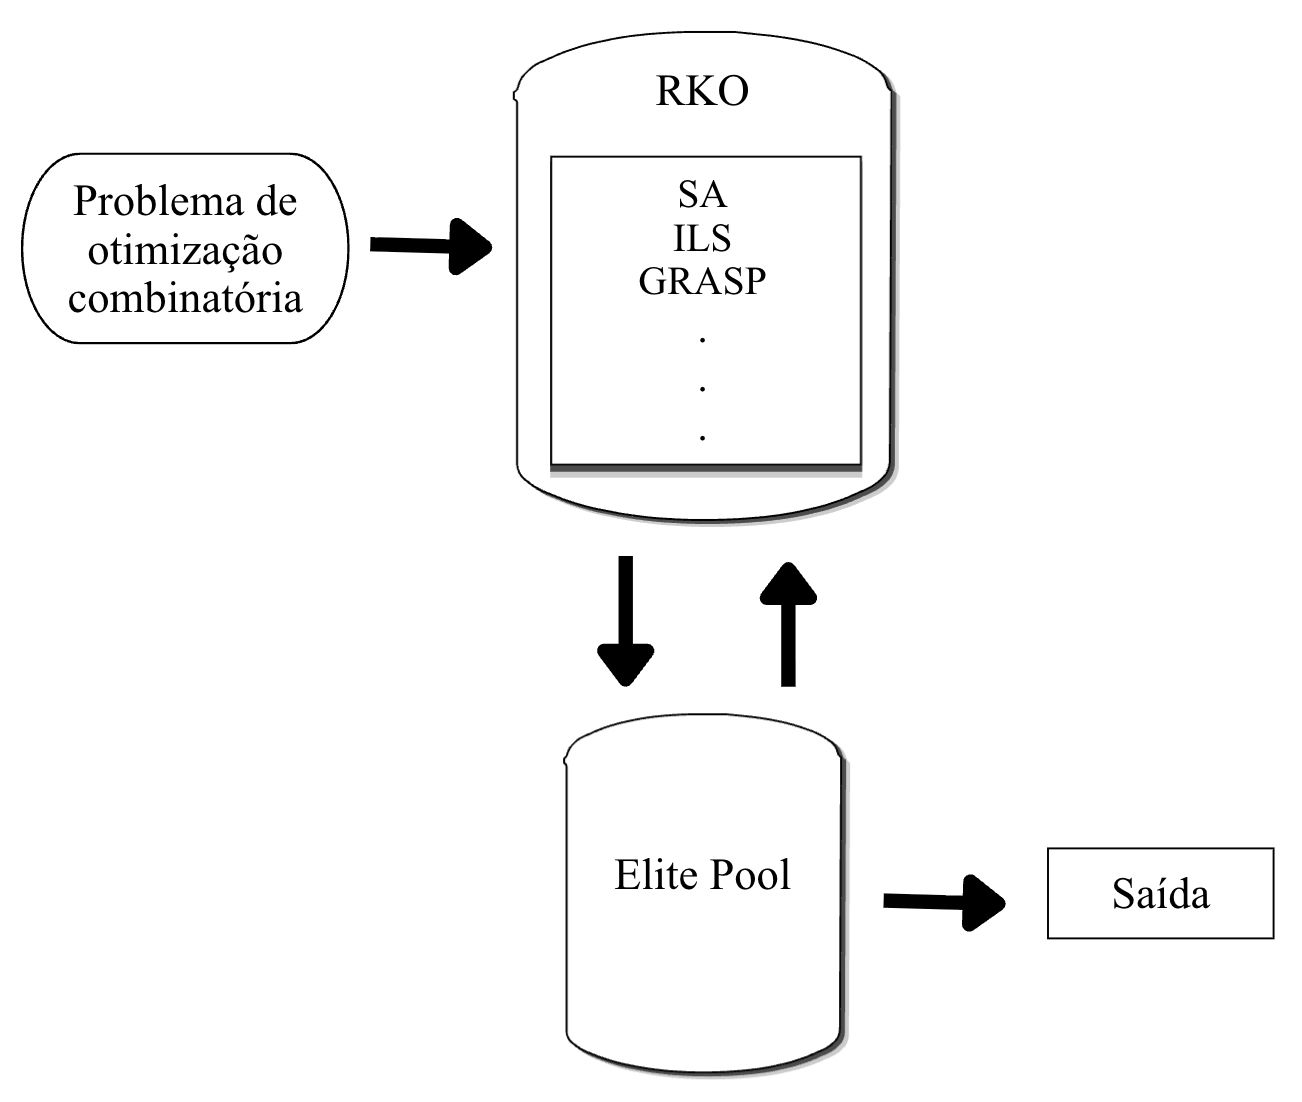
\includegraphics[width=0.6\textwidth]{RKO_FLOW_V2.jpeg}
    \label{fig:RKO_Flow}
\end{figure}

\subsection{Formulações matemáticas da literatura}

Nesta seção, é apresentado duas formulações de PLIM desenvolvidas para o PCmin proposto por Catabriga~\cite{catabriga2025}. Conforme demonstrado no Teorema 2 do referido trabalho, o espaço de busca dos preços pode ser significativamente reduzido sem perda de otimalidade, restringindo-se ao conjunto de preços candidatos. Tal resultado é fundamental, pois permite limitar o domínio das variáveis de preço a um conjunto finito e relevante, reduzindo o tamanho das formulações e melhorando sua tratabilidade computacional.

\subsubsection{Formulação de Decisão Indireta Binária}

A formulação de Decisão Indireta Binária (DIB) foi proposta originalmente por Aggarwal et al.~\cite{aggarwal2004} para o PCmax e posteriormente adaptada por Catabriga~\cite{catabriga2025} para o contexto do PCmin, a formulação DIB baseia-se em decisões indiretas. Nela, os preços são representados explicitamente pelas variáveis binárias $x_{ip}$ (que assume valor 1 se o item $i$ recebe o preço $p$) e $y_{bp}$ (que indica se o comprador $b$ realiza uma compra pagando o valor $p$). Nesse modelo, a escolha do consumidor é inferida a partir do comportamento de pagamento, eliminando a necessidade de modelar diretamente a alocação entre itens e compradores.

\begin{align}
\text{maximizar} \quad & \sum_{b \in B} \sum_{p \in P} p \cdot y_{bp} \label{dib_obj} \\
\text{sujeito a} \quad & \sum_{p \in P} x_{ip} &&\leq 1, && \forall i \in I \label{dib_1} \\
& y_{bp} &&\leq \sum_{i \in I: p \leq v_{ib}} x_{ip}, && \forall b \in B, \forall p \in P \label{dib_2} \\
& \sum_{p \in P} y_{bp} &&\leq 1, && \forall b \in B \label{dib_3} \\
& \sum_{p' \in P: p' < p, p' \leq v_{ib}} x_{ip'} &&\leq 1 - y_{bp}, && \forall b \in B, \forall i \in I, \forall p \in P \label{dib_pcm} \\
& y_{bp}, x_{ip} &&\in \{0, 1\}, && \forall b \in B, \forall i \in I, \forall p \in P \label{dib_dom}
\end{align}

A função objetivo \eqref{dib_obj} maximiza a receita total somando os valores pagos por comprador. A restrição \eqref{dib_1} garante que cada item receba no máximo um preço, enquanto a restrição \eqref{dib_3} limita cada comprador a no máximo uma compra, atendendo à hipótese de demanda unitária.

O vínculo lógico entre preços e compras é estabelecido pelas restrições \eqref{dib_2} e \eqref{dib_pcm}. A restrição \eqref{dib_2} assegura que um comprador só pague o valor $p$ se houver algum item disponível e viável nessa faixa de preço. Por fim, a restrição \eqref{dib_pcm} adapta a formulação ao PCmin ao impor que, se o comprador $b$ pagar o preço $p$, não pode existir nenhum outro item viável com valor estritamente menor. Esse conjunto força o pagamento a corresponder à opção mais barata disponível, representando a dinâmica de escolha do problema sem a necessidade de rastrear explicitamente o item adquirido. Por fim, as restrições de domínio \eqref{dib_dom} definem a natureza binária das variáveis de decisão. 

\subsubsection{Formulação de Decisão Direta}

A formulação de Decisão Direta (DD) baseia-se no modelo linear inteiro misto de Heilporn et al.~\cite{heilporn2010} para precificação livre de inveja, adaptado por Catabriga~\cite{catabriga2025} para o PCmin. Essa abordagem define as variáveis binárias $x_{ib}$ (alocação) e $y_{ib}$ (viabilidade), as variáveis contínuas $\pi_i$ (preço do item) e $\hat{p}_{ib}$ (valor pago), além do conjunto $S_b = \{i \in I \mid v_{ib} > 0\}$ de itens de interesse de cada comprador. Além disso, são definidos os parâmetros limitantes $R_b$ e $\epsilon$. O parâmetro $R_b$ corresponde à maior valoração atribuída pelo comprador $b$ a um item viável, isto é, $R_b = \max\{v_{ib} \mid i \in S_b\}$. Por sua vez, $\epsilon$ representa a menor diferença positiva de preço dentre todas as valorações oferecidas, sendo definido como $\epsilon = \min\{v_{ib} - v_{i'b'} \mid \forall i,i' \in I,\; b,b' \in B,\; v_{ib} \neq v_{i'b'}\}$.

\begin{align}
\text{maximizar} \quad & \sum_{b \in B} \sum_{i \in S_b} \hat{p}_{ib} \label{dd_obj} \\
\text{sujeito a} \quad & \sum_{i \in S_b} x_{ib} &&\leq 1, &&\forall b \in B \label{dd_1} \\
& v_{ib} \cdot x_{ib} - \hat{p}_{ib} &&\geq 0, &&\forall b \in B, \forall i \in S_b \label{dd_2} \\
& \hat{p}_{ib} &&\leq \pi_i, &&\forall b \in B, \forall i \in S_b \label{dd_3} \\
& \hat{p}_{ib} &&\geq \pi_i - R_i \cdot (1 - x_{ib}), &&\forall b \in B, \forall i \in S_b \label{dd_4}  \\
& y_{ib} &&\geq \frac{v_{ib} - \pi_i + \epsilon}{v_{ib} + \epsilon}, &&\forall b \in B, \forall i \in S_b \label{dd_viab}  \\
& \pi_i &&\geq \sum_{j \in S_b} \hat{p}_{jb} - R_b(1 - y_{ib}), &&\forall b \in B, \forall i \in S_b \label{dd_pcm}  \\
& \hat{p}_{ib} &&\geq 0, &&\forall b \in B, \forall i \in S_b \label{dd_5} \\
& \pi_i &&\geq 0, &&\forall i \in I \label{dd_6}  \\
& x_{ib}, y_{ib} &&\in \{0, 1\}, &&\forall b \in B, \forall i \in S_b \label{dd_7} 
\end{align}

A função objetivo \eqref{dd_obj} maximiza a receita total a partir do somatório dos pagamentos $\hat{p}_{ib}$. Em seguida, a restrição \eqref{dd_1} garante a hipótese de demanda unitária, limitando cada comprador a no máximo uma aquisição em $S_b$, enquanto \eqref{dd_2} assegura que nenhum pagamento exceda a valoração máxima do cliente ($R_b$).

O vínculo entre preços e faturamento é estabelecido pelas restrições \eqref{dd_3} e \eqref{dd_4}. Através do parâmetro limitante $R_i$, esse conjunto força que o valor pago $\hat{p}_{ib}$ seja exatamente igual ao preço do item $\pi_i$ sempre que houver alocação ($x_{ib} = 1$), permitindo valor nulo caso contrário. Na sequência, a restrição \eqref{dd_viab} ativa o indicador binário $y_{ib}$ sempre que o preço do item for compatível com a disposição a pagar do comprador, utilizando o parâmetro $\epsilon$ para garantir a precisão dessa escolha.

Por fim, a condição de compra mínima é modelada pela restrição \eqref{dd_pcm}. Quando um item é viável ($y_{ib} = 1$), o modelo impõe que seu preço $\pi_i$ seja limitante superior para o valor pago por $b$. Como o objetivo é maximizar a receita, o sistema é induzido a igualar o pagamento ao menor preço dentre todas as alternativas viáveis para o comprador. Finalmente, as restrições \eqref{dd_5}, \eqref{dd_6} e \eqref{dd_7} definem a não-negatividade e a natureza binária das variáveis.













































 
\section{Objetivos}










O presente trabalho tem como objetivo principal investigar e propor melhorias nas formulações matemáticas existentes para o Problema de Compra Mínima, focando no fortalecimento dos modelos e na sua eficiência computacional. Busca-se desenvolver variações das formulações apresentadas que resultem em modelos com uma relaxação linear mais forte e, consequentemente, mais eficientes quando resolvidos por \emph{solvers} de otimização modernos.

Nesse contexto, pretende-se analisar as formulações DIB e DD para identificar fragilidades, redundâncias ou oportunidades de melhoria. Esse processo será feito por meio da eliminação de simetrias, da redução do número de variáveis e restrições, e da introdução de novas desigualdades quando necessário. Portanto, o objetivo é obter modelos que apresentem melhor desempenho prático em \emph{solvers} como o Gurobi~\cite{gurobi}, reduzindo o tempo de execução e melhorando a qualidade dos limites matemáticos obtidos.

Adicionalmente, este trabalho visa abordar o desafio da escalabilidade, propondo abordagens heurísticas capazes de lidar com instâncias de grande porte, especialmente aquelas que envolvem mais de mil itens ou compradores. Para isso, serão desenvolvidas e avaliadas heurísticas baseadas nas abordagens BRKGA~\cite{Resende2013} e RKO~\cite{Chaves2023}, explorando sua capacidade de produzir soluções de boa qualidade em tempos computacionais reduzidos.

Por fim, espera-se que a combinação entre as melhorias nos modelos matemáticos e o desenvolvimento de métodos heurísticos contribua para ampliar a aplicabilidade prática do problema estudado, permitindo a resolução eficiente de instâncias de grande porte que atualmente são desafiadoras para os métodos exatos tradicionais. 
\section{Plano de Trabalho e Cronograma de atividades}

















O plano de trabalho deste projeto contempla o cumprimento das disciplinas obrigatórias do programa de pós-graduação e o desenvolvimento das etapas de pesquisa ao longo de 2026 e 2027. O primeiro ano será focado na base teórica e acadêmica: os créditos em disciplinas serão cumpridos ao longo de todos os trimestres de 2026, em paralelo com uma revisão bibliográfica inicial nos dois primeiros trimestres para fundamentar o estado da arte do problema. No terceiro trimestre de 2026, o candidato realizará o Exame de Qualificação de Mestrado (EQM) para validar formalmente as definições e modelagens iniciais com a banca. Ainda nesse período, entre o terceiro e o quarto trimestres, o aluno participará do Programa de Estágio Docente (PED), adquirindo experiência prática em docência no ensino superior.

No âmbito do desenvolvimento científico, o final do primeiro ano e o início do segundo consolidarão a parte exata e a internacionalização da pesquisa. As melhorias nas formulações matemáticas (DIB e DD) ocorrerão entre o terceiro e o quarto trimestres de 2026. Em seguida, nos dois primeiros trimestres de 2027, está prevista a realização de um estágio de pesquisa no exterior por meio do programa de Bolsa Estágio de Pesquisa no Exterior (BEPE). Esse período será fundamental para aprofundar os aspectos teóricos do PCmin e abrir frentes de colaboração internacional. Para o desenvolvimento dessa etapa, pretende-se cooperar com pesquisadores relevantes da área, tais como Manuel Iori (\emph{University of Modena and Reggio Emilia}), Martine Labbé (\emph{Université Libre de Bruxelles}), Levent Tuncel e Tor Gunnar Josefsson Myklebust (\emph{University of Waterloo}).

O restante do segundo ano será dedicado à vertente heurística, testes e finalização da escrita. Durante o primeiro semestre de 2027, serão desenvolvidos os algoritmos baseados em BRKGA e RKO. A etapa de experimentação computacional e análise de desempenho acontecerá no terceiro trimestre de 2027, utilizando o solver Gurobi e os algoritmos propostos para validar a eficiência das abordagens. Com os resultados consolidados, o terceiro trimestre também contemplará a preparação de trabalhos científicos para submissão e apresentação em conferências e eventos da área. Por fim, a redação da dissertação de mestrado será conduzida entre o terceiro e o quarto trimestres, culminando na defesa ao final de 2027. A distribuição dessas atividades está detalhada na Tabela~\ref{cronograma}.

\begin{table}[H]
\caption{Cronograma trimestral do projeto de Mestrado}
\label{cronograma}
\centering
\begin{adjustbox}{width=\textwidth}
\begin{tabular}{l ccc ccc cc}
\toprule
 & \multicolumn{4}{c}{\textbf{2026}} & \multicolumn{4}{c}{\textbf{2027}} \\
\cmidrule(r){2-5} \cmidrule(l){6-9}
 & \textbf{Jan-Mar} & \textbf{Abr-Jun} & \textbf{Jul-Set} & \textbf{Out-Dez} & \textbf{Jan-Mar} & \textbf{Abr-Jun} & \textbf{Jul-Set} & \textbf{Out-Dez} \\
\midrule
Disciplinas                   & • & • & • & • &   &   &   &   \\
EQM                           &   &   & • &   &   &   &   &   \\
Revisão bibliográfica        & • & • &  &  &  &  &  &  \\
BEPE                          &   &   &   &   & • & • &   &   \\
PED                           &   &   & • & • &   &   &   &   \\
Melhorias nas formulações     &   &   & • & • &   &   &   &   \\
Desenvolvimento de heurísticas&   &   &   &   & • & • &   &   \\
Experimentação computacional  &   &   & • & • & • & • & • &   \\
Escrita de artigos científicos&   &   &   &   &   &   & • &   \\
Escrita da dissertação        &   &   &   &   &   &   & • & • \\
Entrega da dissertação e defesa&  &   &   &   &   &   &   & • \\
\bottomrule
\end{tabular}
\end{adjustbox}
\end{table} 
\section{Materiais e Métodos}

O presente projeto será desenvolvido nas dependências do Laboratório de Otimização e Combinatória (LOCo) do Instituto de Computação, um ambiente compartilhado com outros estudantes de mestrado e doutorado que propicia a troca de ideias e a colaboração científica. Os algoritmos propostos serão testados empiricamente. Devido ao grande volume de instâncias disponíveis na literatura e aos elevados limites de tempo comumente adotados em trabalhos anteriores (frequentemente estabelecidos em uma hora por execução), as baterias de testes podem demandar dias para serem concluídas. Por essa razão, os experimentos computacionais serão executados nos servidores de alto desempenho disponibilizados pelo LOCo.

Para o suporte teórico e o levantamento do estado da arte, o candidato utilizará o acervo bibliográfico físico da biblioteca do Instituto de Matemática, Estatística e Computação Científica, além do Portal de Periódicos da CAPES, que assegura acesso institucional e gratuito às principais revistas científicas da área para os estudantes da Unicamp.

A metodologia de acompanhamento incluirá reuniões entre o candidato e o orientador para debater o andamento da pesquisa, superar desafios metodológicos e alinhar novas estratégias de resolução. Adicionalmente, encontros com os demais membros do grupo de pesquisa do orientador ocorrerão de forma periódica ou sob demanda, promovendo a integração e a discussão coletiva dos resultados alcançados. 
\section{Forma de Análise dos Resultados}













A análise dos resultados deste trabalho será conduzida de forma sistemática para avaliar a qualidade e a eficiência das formulações e dos métodos de solução desenvolvidos. A investigação vai considerar tanto o valor das soluções obtidas quanto o desempenho computacional dos algoritmos diante de instâncias com diferentes características.

Inicialmente, as formulações matemáticas serão avaliadas por sua capacidade de produzir soluções ótimas ou limites de alta qualidade dentro de tempos preestabelecidos. Serão analisadas métricas como o valor da função objetivo, o tempo de processamento e o número de nós explorados na árvore de busca. Além disso, será verificada a consistência dos modelos em cenários de diferentes dimensões, com ênfase especial em problemas de grande porte. Para a comparação entre as diferentes formulações, será utilizada a metodologia de \emph{performance profiles} de Dolan e Moré~\cite{Dolan2002}. Essa técnica compara o desempenho relativo dos métodos por meio de curvas de distribuição acumulada, mostrando a probabilidade de um modelo resolver uma instância dentro de um fator múltiplo do tempo do método mais rápido. Isso permite identificar a eficiência e a resiliência geral de cada abordagem.

No âmbito das meta-heurísticas (BRKGA e RKO), a qualidade das soluções será confrontada com os resultados dos métodos exatos por meio do cálculo do gap de otimalidade, utilizando os limites inferiores obtidos pelos modelos matemáticos. Para avaliar o comportamento estocástico dessas heurísticas, será usada a metodologia de \emph{Time-to-Target plots}~\cite{aiex2007}. Essa ferramenta mostra a probabilidade empírica de o algoritmo encontrar uma solução tão boa quanto um valor-alvo em função do tempo computacional, o que ajuda a caracterizar a velocidade de convergência e a estabilidade dos métodos propostos.

Por fim, as análises comparativas e críticas serão consolidadas em artigos científicos e na dissertação de mestrado, buscando identificar padrões de desempenho, limitações e direções para investigações futuras. 


\newpage

\begingroup
\footnotesize
\setlength{\columnsep}{1em}
\begin{multicols}{2}
\printbibliography
\end{multicols}
\endgroup

\end{document}